\documentclass[a4paper,12pt]{article}

\usepackage[utf8]{inputenc}
\usepackage{graphicx}
\usepackage{amsmath}
\usepackage[serbian]{babel}
\usepackage{url}
\usepackage[T1]{fontenc}
\usepackage{lmodern}
\usepackage{float}

\usepackage{listings}
\usepackage{xcolor}

\lstset{
    language=Python,
    basicstyle=\ttfamily\small,
    keywordstyle=\color{blue},
    commentstyle=\color{gray}\itshape,
    stringstyle=\color{red},
    numbers=left,
    numberstyle=\tiny\color{gray},
    stepnumber=1,
    numbersep=5pt,
    showstringspaces=false,
    breaklines=true,
    frame=single,
}

\renewcommand{\figurename}{Slika}  % Change "Figure" to "Slika"
\renewcommand{\tablename}{Tabela}
\begin{document}

\begin{titlepage}
    \centering
	\begin{figure}[htbp]
    	\centering
    	
\includegraphics[width=0.4\textwidth]{images/logo.png}
	\end{figure}
    { Univerzitet u Beogradu \\ Matematički fakultet\par}
	
    \vfill

    {\Large \textbf{Seminarski rad}\par}

    \vspace{1cm}

    {\Large \textbf{Primena n-gramske analize na amino-kiselinske i nukleotidne kodove}\par}

    \vfill

    
	
	
	\begin{tabbing}
	\hspace{10cm} \= \hspace{10cm} \= \kill
	\textbf{Mentor:} \>  \textbf{Studenti:} \\
	Prof. dr Nenad Mitić \> Iva Milutinović 262/2021 \\
	Katedra za računarstvo i informatiku \> Jovana Urošević 189/2021 \\
	\> Smer: Informatika
	\end{tabbing}

    \vfill

    \textbf{Datum:} 2024/25

\end{titlepage}
\newpage
\tableofcontents
\newpage
\section{Uvod}
\newpage
\section{Parsiranje podataka i n-gramska analiza}
\textbf{Podaci i izvor:} U cilju klasterovanja i određivanja pravila pridruživanja više vrsta virusa (SARS-CoV-2, MERS, Ebola i Marburg), prikupljeni su sekvencioni podaci sa portala \textbf{NCBI Virus:} \url{https://www.ncbi.nlm.nih.gov/labs/virus/vssi/#/find-data/virus}. Primenjeni su filteri: \textit{ambiguous characters = 0} (isključivo
sekvence bez dvosmislenih simbola) i \textit{nucleotide completeness = complete} (samo kompletni genomi).

Zbog ogromnog broja dostupnih izolata, za SARS-CoV-2 korišćen je ograničen skup tačno određenih
\textit{accession} brojeva, dok su za ostale viruse preuzete sve dostupne kompletne sekvence koje ispunjavaju
zadate kriterijume. U nastavku su opisani koraci parsiranja i obrade podataka za proteinske (amino-
kiselinske) i nukleotidne FASTA fajlove, uključujući n-gramsku analizu i konstrukciju matrica frekvencija koje
su kasnije korišćene za klasterovanje i pravila pridruživanja.

\subsection{Parsiranje amino-kiselinskih FASTA fajlova}

\textbf{Format FASTA fajla:} Proteinske sekvence su preuzete u FASTA formatu, gde je svaka sekvenca
predstavljena zaglavljem i nizom jednoslovnih kodova aminokiselina. Zaglavlje počinje znakom \texttt{>} praćenim
opisom ili identifikatorom sekvence. U primeru FASTA zapisa ispod, zaglavlje sadrži jedinstveni identifikator i opis:

\begin{lstlisting}[language=]
>gi|5524211|gb|AAD44166.1| cytochrome b [Elephas maximus maximus]
LCLYTHIGRNIYYGSYLYSETWNTGIMLLLITMATAFMGYVLPWGQMSFW...
\end{lstlisting}

Ovaj primer ilustrije da zaglavlje često uključuje naziv proteina i naziv organizma u uglastim zagradama. U kontekstu naših podataka, naziv virusa (npr. Ebola virus, SARS-CoV-2) tipično je naveden u zagradama,
dok pre njega stoji naziv proteina (npr. spike glycoprotein, nucleocapsid protein). FASTA fajl može sadržati više
sekvenci (tzv. multi-FASTA format), jedna za drugom, gde svaki zapis počinje svojim \texttt{>} zaglavljem.

\vspace{10pt}
\textbf{Objedinjavanje podataka i mapiranje virusa/proteina:} Preuzete FASTA datoteke (odvojene
po virusima) parsirane su programskim putem i objedinjene u jedinstvenu
strukturu podataka radi dalje obrade. Svaki zapis u strukturi predstavlja jedan virusni protein i čuva sledeće
informacije: (i) identifikator ili naziv virusa, (ii) naziv/tip proteina, i (iii) aminokiselinsku sekvencu. Parsiranje
je ostvareno prolaskom kroz FASTA fajl liniju po liniju: kada se detektuje linija koja počinje sa \texttt{>} tretira se
kao zaglavlje, iz kojeg se ekstrahuju podaci o virusu i proteinu, dok se naredne linije pridružuju sekvenci
proteina. 

\vspace{10pt}
\textbf{Pseudokod za parsiranje FASTA fajlova:}

\begin{lstlisting}
for line in open("virus_proteins.fasta"):
    if line.startswith(">"):
        header = line[1:].strip()
        protein_name = header.split("[")[0].strip()
        virus_name = header.split("[")[1].rstrip("]")
    else:
        seq = line.strip() 
\end{lstlisting}

U gornjem primeru, string iz zaglavlja se deli na deo pre i posle znaka \texttt{[} kako bi se dobili naziv proteina i
naziv virusa. Tako svaki zapis povezujemo sa odgovarajućim virusom i proteinskim produktom. Mapiranje
virusa i proteina rešeno je tako što su nazivi virusa i proteina sačuvani kao posebna polja ili kao deo
jedinstvenog ključa. 

\vspace{10pt}
\textbf{Filtriranje dvosmislenih simbola:} Kako je navedeno, korišćene su sekvence bez neodređenih znakova
(\textit{ambiguous characters = 0}). Ipak, prilikom parsiranja je verifikovano da u amino-kiselinskim sekvencama
ima dvosmislenih kodova poput B, J, O, U, X, Z. Ovi znakovi predstavljaju ili ne-standardne ili neodređene
aminokiseline: npr. B označava asparagin ili asparaginsku kiselinu (Asx), Z glutamin ili glutaminsku kiselinu
(Glx), J leucin ili izoleucin (Xle), X bilo koju aminokiselinu (nepoznatu), dok su O i U specijalni kodovi za
nekanonske aminokiseline pirolizin i selenocistein. Sekvence koje bi sadržale takve simbole bile bi
filtrirane ili označene za izuzimanje kako bi se obezbedilo da analiza n-grame vrši samo nad 20 standardnih
aminokiselina. 

\subsection{N-gramska analiza proteinskih sekvenci}

Za svaku amino-kiselinsku sekvencu generisani su podnizovi
fiksne dužine (n-grami) i izračunate njihove učestalosti. Odabrane su dužine od 3, 4 i 5 (trigrami, tetragrami i
pentagrami) kako bi se uhvatili motivi u proteinskim sekvencama različitih veličina. N-gram analiza je
implementirana kliznim prozorom duž sekvence: za dati n , pomera se prozor od početka do kraja
sekvence i izdvaja svaki podniz dužine n . Broj mogućih različitih n-grama za aminokiselinske sekvence je
velik (maksimalno $20^n$ kombinacija za standardnih 20 aminokiselina), ali se u praksi javljaju samo
podskupovi te liste. Postupak za generisanje i brojanje n-grama po svakoj sekvenci može se opisati sledećim
koracima:

\begin{enumerate}
  \item \textbf{Generisanje n-grama:} za svaki indeks i u sekvenci od 1 do (L–n+1) uzima se podniz seq[i:i+n]
(dužine n). Na primer, za sekvencu "ACDEFGH" i n=3 dobili bismo trigrami: "ACD", "CDE", "DEF",
itd.
  \item \textbf{Brojanje učestalosti:} za svaku sekvencu se vodi rečnik (mapa) ili brojač pojavljivanja n-grama. Svaki
put kada se generiše n-gram, uveća se njegov brojač za tu sekvencu.
  \item \textbf{Skladištenje rezultata:} nakon prolaska kroz celu sekvencu, rezultujući brojači predstavljaju profil
sekvence u prostoru n-grama.
\end{enumerate}

\textbf{Primer generisanja trigram n-grama:}

\begin{lstlisting}
seq = "ACDEFGH"
n = 3
ngrams = [seq[i:i+n] for i in range(len(seq) - n + 1)]
# Rezultat: ["ACD", "CDE", "DEF", "EFG", "FGH"]
\end{lstlisting}

Slično tome, koristeći kolekciju Counter iz biblioteke collections, lako se dobiju frekvencije svakog n-grama
za sekvencu.

\vspace{10pt}
\textbf{Konstrukcija matrice frekvencija:} Nakon što su izračunate frekvencije n-grama za svaku proteinsku
sekvencu, podaci su organizovani u veliku matricu (tabelu), koja je zatim snimljena u CSV formatu radi lakše
analize. U toj matrici svaki red odgovara jednom proteinu (jednoj sekvenci) identifikovanom kombinacijom
virusa i naziva proteina, a svaka kolona odgovara jednom mogućem n-gramu dužine 3, 4 ili 5. Element
matrice $M_{ij}$ predstavlja broj pojavljivanja određenog n-grama j u proteinu i. Kolone su najpre
generisane unijom svih n-grama koji se uopšte pojavljuju u bilo kojoj sekvenci (za dati n), a za sekvence u
kojima neki motiv nije prisutan automatski će vrednost biti 0 u toj koloni. Tako su napravljene tri odvojene
matrice – za trigrame, tetragrame i pentagrame – s tim da svaka sadrži |V| redova (ukupan broj proteinskih
sekvenci svih posmatranih virusa) i $N_{n}$ kolona (broj različitih n-grama dužine n pronađenih u
celom skupu). Ove matrice predstavljaju kvantitativnu numeričku reprezentaciju proteinskih sekvenci,
pogodnu za primenu pravila pridruživanja i klasterovanja.

\subsection{Parsiranje nukleotidnih FASTA fajlova}

\textbf{Specifičnosti genomskih sekvenci:} Za analizu nukleotidnih sekvenci korišćeni su kompletni genomi virusa
iz iste grupe (SARS-CoV-2, MERS-coronavirus, različiti Ebolavirus i Marburgvirus). FASTA fajlovi za genome
sličnog su formata kao proteinski, ali zaglavlja obično sadrže naziv virusa i često sam \textit{accession} broj
bez posebnog naziva gena (jer je sekvenca čitav virusni genom). Na primer, zaglavlje može izgledati:

\begin{lstlisting}[language=]
>NC_002549 Marburg virus isolate Musoke, complete genome
\end{lstlisting}

Parsiranje ovih fajlova obavljeno
je slično kao za proteine – čitanjem svake linije i izdvajanjem meta-podataka iz zaglavlja. Iz svakog zaglavlja
izolovan je naziv virusa (npr. "Marburg virus", "Bombali ebolavirus", "SARS-CoV-2"), dok je cela naredna sekvenca (koja može imati i više hiljada nukleotida) sačuvana kao
string. U strukturi podataka, svaki zapis je predstavljao jedan genom, povezan sa svojim virusom (i
sojem), što omogućava da se kasnije rezultati grupišu po tipovima virusa.

\vspace{10pt}
\textbf{Filtriranje nevalidnih nukleotidnih simbola:} Kao i kod proteina, osigurano je da nukleotidne sekvence ne
sadrže dvosmislene kodove. Standardna nukleotidna abeceda obuhvata samo A, C, G, T (U), dok su ostala
slova deo IUPAC oznaka za neodređene baze. U takve spadaju: B, D, H, K, M, R, S, V, W, Y, N, koje
označavaju višestruke ili nepoznate nukleotide (npr. N znači bilo koja baza; R znači purina A/G; Y pirimidina
C/T; K = G/T, itd.). U procesiranju je urađena provera
te se svi nedozvoljeni simboli uklanjaju, jer bi u suprotnom narušili tačnost n-
gram analize (npr. podniz "ACNGA" ne može se smatrati validnim 5-merom zbog 'N').

\subsection{N-gramska analiza nukleotidnih sekvenci}

Za poređenje celih genoma, korišćena je analiza frekvencije
dužih n-grama dužine 6, 7, 8 i 9. Razlog za izbor ovih dužina je što kraći n-grami(poput
tri- ili pet-nukleotidnih) mogu biti manje informativni zbog kratkih ponavljajućih motiva i ograničene
kombinatorike ($4^3 = 64$
 mogućih trinukleotida), dok duži n-grami pružaju ekspresivniji "potpis"
genomske sekvence. Postupak generisanja 6–9-grama identičan je onome opisanom za proteine: za svaki
genom, prolazi se duž niza nukleotida i prave se svi podnizovi dužine n, nakon čega se broje pojavljivanja. Svaki genom dužine L sadržaće (L–n+1) n-grama dužine. Broj mogućih različitih n-grama
eksponencijalno raste sa n. Za DNA abecedu od 4 slova: \begin{itemize}
    \item $4^6 = 4096$ mogućih 6-mer podnizova
    \item $4^9 = 262144$ mogućih 9-mer podnizova
\end{itemize}
U
implementaciji, za svaki od izabranih n vrednosti generisana je posebna frekventna distribucija za dati
genom.

\vspace{10pt}
\textbf{Kreiranje matrica po virusima:} S obzirom da su genomske sekvence duže i da se skupovi sekvenci
razlikuju po virusima, frekvencije n-grama su inicijalno računane odvojeno za svaki virusni skup. Za svaki virus
(npr. za sve sekvence SARS-CoV-2, posebno za sve sekvence ebolavirusa itd.) formirana je matrica gde su
redovi pojedinačni genomski izolati tog virusa, a kolone predstavljaju n-gram frekvencije. U svaku matricu
uključeni su svi n-grami dužine n koji su se pojavili u barem jednom genomu posmatranog virusa, pri čemu
su za sekvence koje ih ne sadrže vrednosti 0. Nakon što su generisane takve matrice za svaki virus posebno,
one su po potrebi spojene zajedno kako bi se omogućilo poređenje između različitih virusa.
Sličan pristup sačuvan je kao kod proteina: izrađene su posebne matrice za 6-mer, 7-mer, 8-mer i 9-mer
analize. Svaka matrica ima onoliko redova koliko je genoma uzeto u obzir za dati virus, a kolona onoliko
koliko ima različitih n-grama te dužine u celom skupu. Ove CSV matrice predstavljaju kvantitativne
karakteristike genoma i čine osnovu za dalju analizu sličnosti sekvenci.


\newpage
\section{Klasterovanje}

\subsection{SOM (Self-Organizing Map)}
\textbf{SOM (Self-Organizing Map)} ili samoorganizujuća mapa je algoritam neuronskih mreža koji koristi neurone bez nadzora (unsupervised learning) kako bi izvršio projekciju visokodimenzionalnih podataka u dvodimenzionalni prostor, uz očuvanje topoloških relacija između ulaznih podataka.

Glavna prednost SOM-a jeste što ne zahteva prethodno definisane klase, već sam organizuje podatke na osnovu njihove sličnosti i strukture.

SOM mapira slične ulazne vektore na bliske pozicije na mreži neurona (najčešće 2D mreža), čime omogućava vizualnu i analitičku interpretaciju klastera. Tipično se koristi u bioinformatici, prepoznavanju obrazaca, genomskoj klasifikaciji, vizuelizaciji kompleksnih podataka i detekciji anomalija.

\textbf{Način funkcionisanja Self-Organizing Map algoritma:}SOM se sastoji od dvodimenzionalne mreže neurona, gde svaki neuron ima svoj vektor težina iste dimenzije kao ulazni podaci. Algoritam prolazi kroz sledeće korake:

\begin{enumerate}
  \item \textbf{Inicijalizacija težina:} Nasumično ili linearnom interpolacijom.
  \item \textbf{Poređenje:} Za svaki ulazni vektor određuje se neuron čiji je vektor težina najsličniji ulazu (tzv. BMU – Best Matching Unit).
  \item \textbf{Ažuriranje težina:} Težine BMU-a i njegovih suseda u mreži se ažuriraju tako da se približe ulaznom vektoru. Promene su kontrolisane koeficijentom učenja i funkcijom susedstva.
  \item \textbf{Iteracija:} Postupak se ponavlja za sve ulazne vektore i tokom više epoha. Tokom vremena se smanjuju koeficijent učenja i širina susedstva.
\end{enumerate}

\textbf{Primena SOM-a u kontekstu naše analize:} U analizi viralnih sekvenci, radimo sa vektorima visokih dimenzija koji predstavljaju frekvencije n-grama u genomskim i proteinskim sekvencama. Takvi vektori nisu lako interpretabilni niti vizuelizovani u 2D prostoru. SOM je idealan za ovaj zadatak iz nekoliko razloga:
\begin{itemize}
    \item Preslikava složene podatke u 2D prostor, što omogućava jednostavnu vizualizaciju.
    \item Zadržava sličnost – sekvence sa sličnim n-gram profilima biće mapirane u blizini.
    \item Ne zahteva unapred poznat broj klasa ili oznake (klasteruje bez nadzora).
    \item Omogućava detekciju grupacija među sekvencama različitih virusa i proteina.
\end{itemize}

\textbf{Parametri SOM algoritma koje smo koristile:}
\begin{itemize}
    \item Dimenzije mreže(som\_x, som\_y): 15x15 neurona(225 neurona u mreži)
    \item Broj iteracija: 1000 (broj epoha treniranja)
    \item Funkcija udaljenosti: Euklidska distanca
    \item Koeficijent učenja: 0.5
    \item Širina susedstva (sigma): 1.0
\end{itemize}

Ovi parametri su podešeni tako da omoguće postepenu konvergenciju mreže ka stabilnim klasterima i jasnu topološku strukturu među sekvencama.

\vspace{10pt}
\textbf{SOM nad amino-kiselinskim sekvencama}
\vspace{10pt}

Kod amino-kiselinskih sekvenci koristile smo već prethodno generisane n-gram matrice (n = 3, 4, 5), gde je svaka sekvenca predstavljena kao vektor frekvencija n-grama. Ove matrice su sadržavale i dodatne kolone sa oznakama:

\begin{itemize}
    \item virus\_type – oznaka virusa (npr. SARS-CoV-2, Marburg virus)
    \item protein\_type – oznaka proteina (npr. GP, spike, E protein)
\end{itemize}

Kako bismo istražile strukturu podataka, SOM algoritam je pokrenut dva puta:
\begin{enumerate}
  \item \textbf{Grupisanje prema tipu virusa}
  \item \textbf{Grupisanje prema tipu proteina} 
\end{enumerate}

U oba slučaja, oznake (`virus\_type` ili `protein\_type`) nisu korišćene u učenju mreže, već samo u bojenju rezultata, kako bismo proverile da li SOM klasteri odgovaraju biološkim kategorijama.

Podaci su standardizovani pomoću StandardScaler() – čime su sve vrednosti vektora n-gram frekvencija skalirane na istu skalu (normalizovane), što je ključno za stabilan rad SOM algoritma.

\textbf{Vizualizacije i interpretacija:}
Koristile smo dve vrste vizualizacija za svaku n-gram kombinaciju:
\begin{enumerate}
  \item \textbf{U-Matrix (distance map):} Prikazuje razdaljine između susednih neurona na mapi. Tamnije oblasti predstavljaju veće razlike između susednih neurona i ukazuju na granične linije između klastera.
  \item \textbf{Mapa neurona sa tačkama:} Sekvence su predstavljene tačkama, mapirane na pozicije njihovih BMU neurona i obojene prema tipu virusa ili proteina.
\end{enumerate}

\begin{figure}[h!]
    \centering
    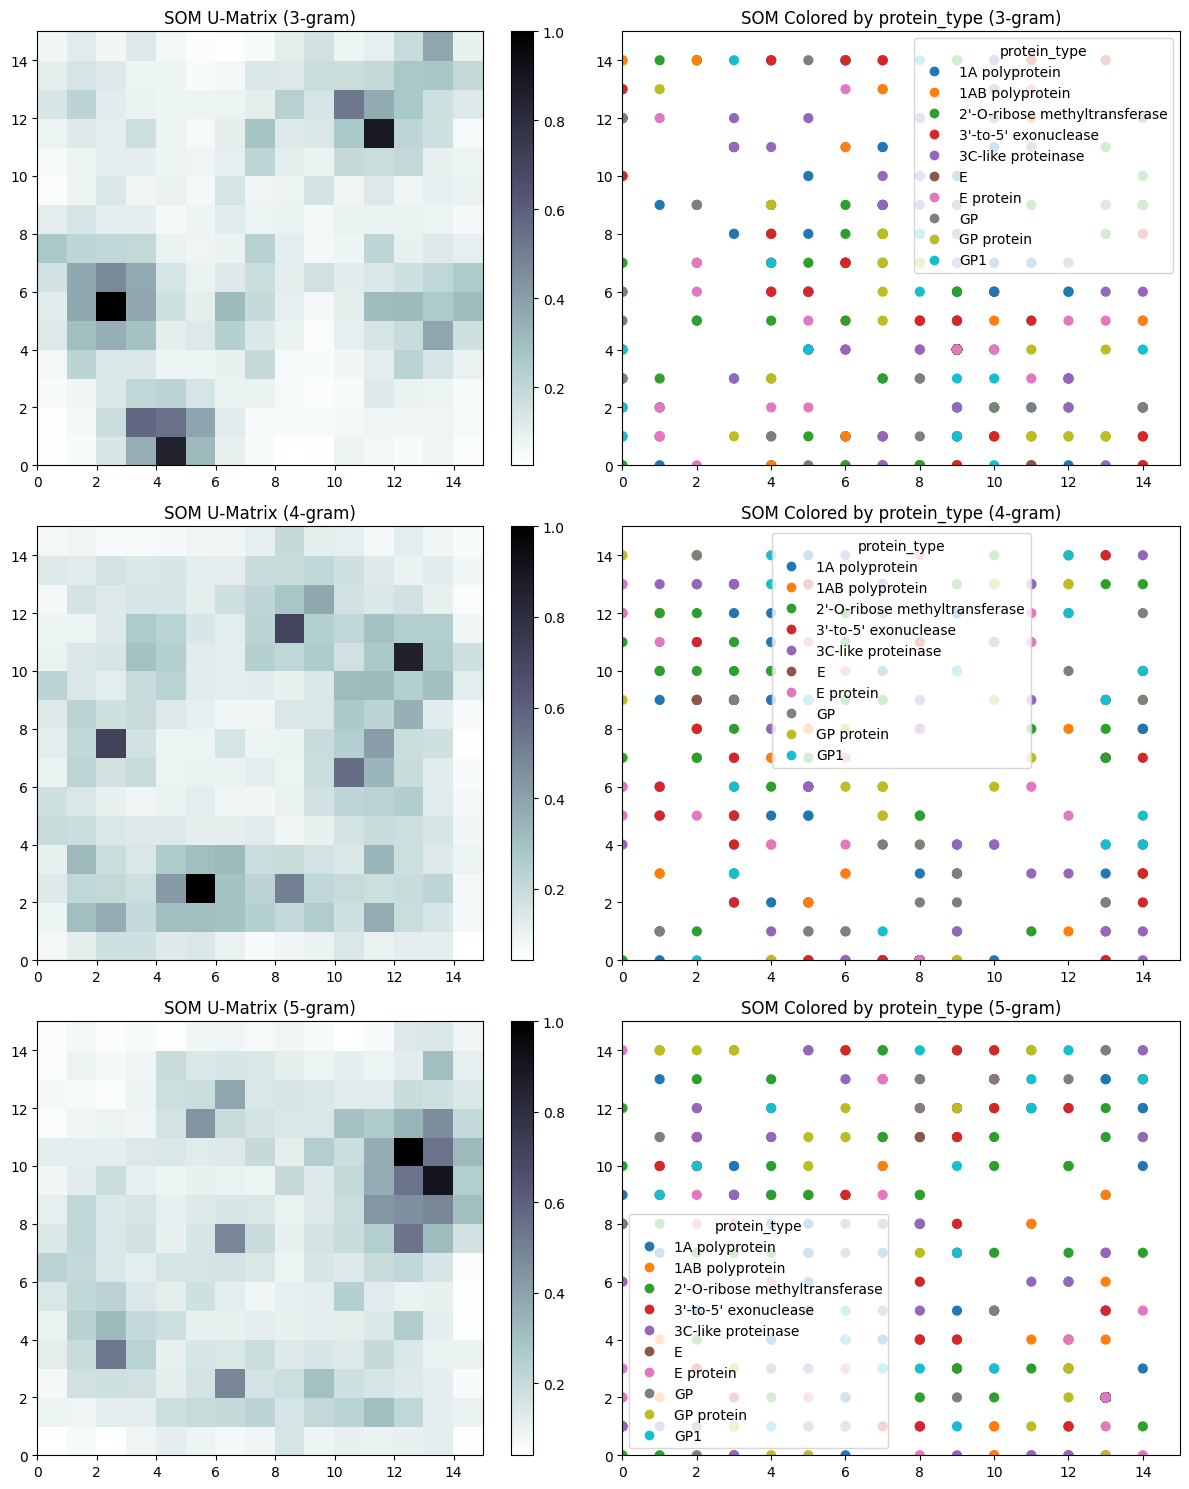
\includegraphics[width=0.5\textwidth]{images/som-amino-acid-protein.png}
    \caption{Vizualizacija za grupisanje prema tipu proteina}
    \label{fig:som-struktura3}
\end{figure}

\textbf{Diskusija rezultata:}
SOM mreža identifikovala je veliki broj klastera (132–171), što ukazuje na visoku raznovrsnost sekvenci i izražene razlike u n-gram profilima između različitih virusa i proteina. Neke ključne opservacije:

\begin{itemize}
    \item Povećanjem n-gram dužine sa 3 na 5, broj klastera raste – to je očekivano jer duži n-grami bolje diferenciraju sekvence, ali istovremeno povećavaju sparsenost podataka.
    \item Klasteri se često grupišu po tipu virusa – što pokazuje da sekvence virusa istog tipa imaju slične n-gram profile.
    \item Grupisanje po tipu proteina otkriva klastere gde različiti virusi proizvode funkcionalno slične proteine – npr. spike proteini iz različitih koronavirusa su često blizu na mapi.
\end{itemize}

Broj BMU klastera koji su različiti (tj. unikatne pozicije na SOM mapi koje su bile aktivne) predstavlja broj funkcionalno različitih grupa koje je mreža detektovala. Veći broj klastera može ukazivati i na visoku rezoluciju mreže, ali i na kompleksnost podataka.

\begin{figure}[h!]
    \centering
    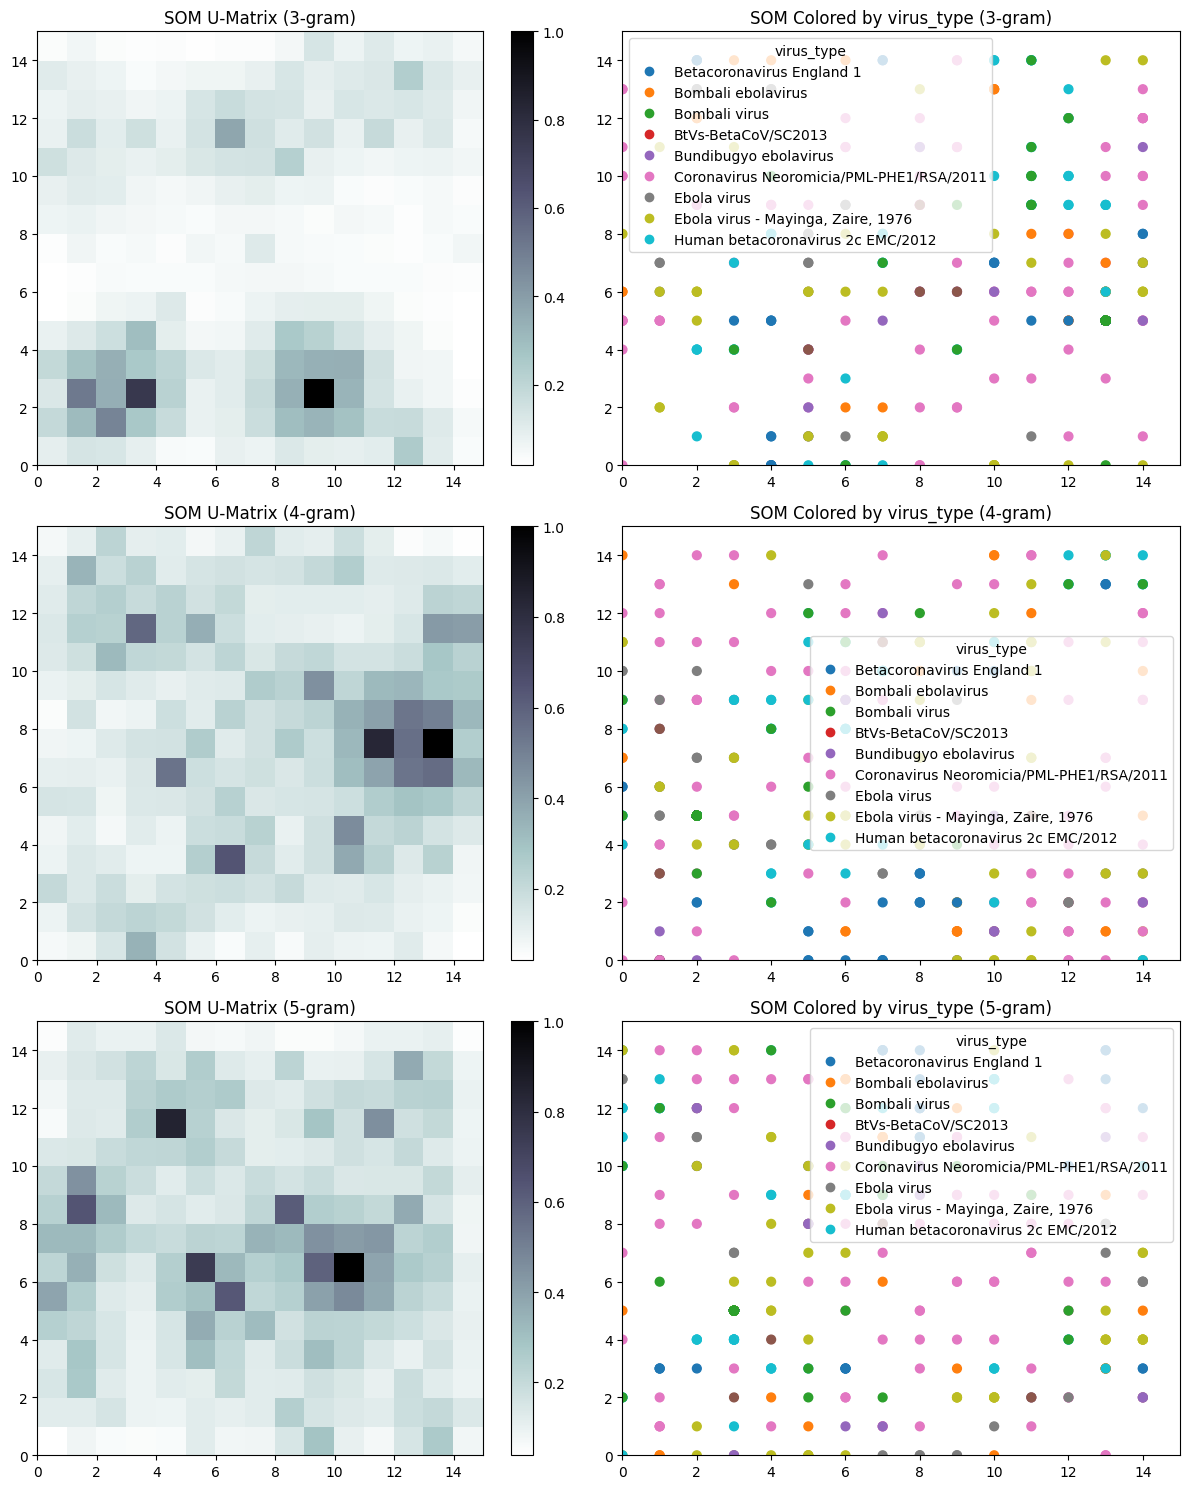
\includegraphics[width=0.5\textwidth]{images/som-amino-acid-virus.png}
    \caption{Vizualizacija za grupisanje prema tipu virusa}
    \label{fig:som-struktura2}
\end{figure}

\textbf{Slika 1 i 2:} Primer rezultata samoorganizujuće mape za proteinske sekvence (3-gram frekvencije
aminokiselina). Prikazana je U-matrica SOM mreže, gde tamnija boja označava veće rastojanje između
neurona (granične oblasti klastera). Preko toga je izvršeno bojenje po vrsti virusa čiji protein pripada
datom neuronu. Vidljivo je grupisanje proteina istog virusa u zajedničke klastere (npr. proteini ebolavirusa
grupisani zajedno, odvojeni od koronavirusnih proteina), što ukazuje da i prostori 3-grama nose filogenetski
signal za razlikovanje virusa. Slični rezultati dobijeni su i za 4-gram i 5-gram frekvencije, što dodatno potvrđuje stabilnost ovog pristupa. Na tamnijim mestima SOM mape primećuje se nedostatak sekvenci, dok je u drugim delovima jasno uočljivo kako su klasteri međusobno razdvojeni.

\vspace{20pt}
\textbf{SOM nad nukleotidnim sekvencama}
\vspace{10pt}

Za nukleotidne sekvence korišćene su n-gram matrice za dužine 6, 7, 8 i 9, izgrađene na osnovu kompletnih genoma virusa. Svaki red u matrici predstavlja jedan genom (izolat), dok su kolone različiti n-grami. Pošto se ovde radi o dužim sekvencama sa više stabilnih obrazaca, korišćeni su i duži n-grami nego kod proteina. Oznaka `virus\_type` se koristila kao labela za bojenje tačaka.

\vspace{10pt}
\textbf{Vizualizacije i interpretacija:}
Koristile smo iste dve vizualizacije:
\begin{enumerate}
  \item \textbf{U-Matrix (distance map):} Za identifikaciju granica između klastera.
  \item \textbf{Mapa neurona sa tačkama:} Svaka sekvenca je prikazana kao tačka, bojena prema virusu (npr. SARS-CoV-2, Ebola virus), čime se uočava grupisanje genoma po virusnim vrstama.
\end{enumerate}

\textbf{Diskusija rezultata:}
Za razliku od amino-kiselinskih podataka, SOM mreža je za sve nukleotidne n-grame proizvela konzistentan broj od 28 klastera. Ovaj broj veoma verovatno odgovara broju različitih virusnih izolata ili grupacija, što ukazuje da:

\begin{itemize}
    \item Genomske sekvence su znatno homogenije unutar iste vrste, ali dovoljno različite među vrstama da ih SOM može jasno razdvojiti.
    \item SOM je detektovao jasne evolutivne i taksonomske granice između genoma virusa (npr. između ebolavirusa i koronavirusa).
    \item Za razliku od proteinskih sekvenci koje imaju veću unutrašnju raznovrsnost (različiti proteini jednog virusa), kompletni genomi se ponašaju kao stabilniji entiteti, pa su i rezultati klasterovanja stabilniji.
\end{itemize}

\begin{figure}[h!]
    \centering
    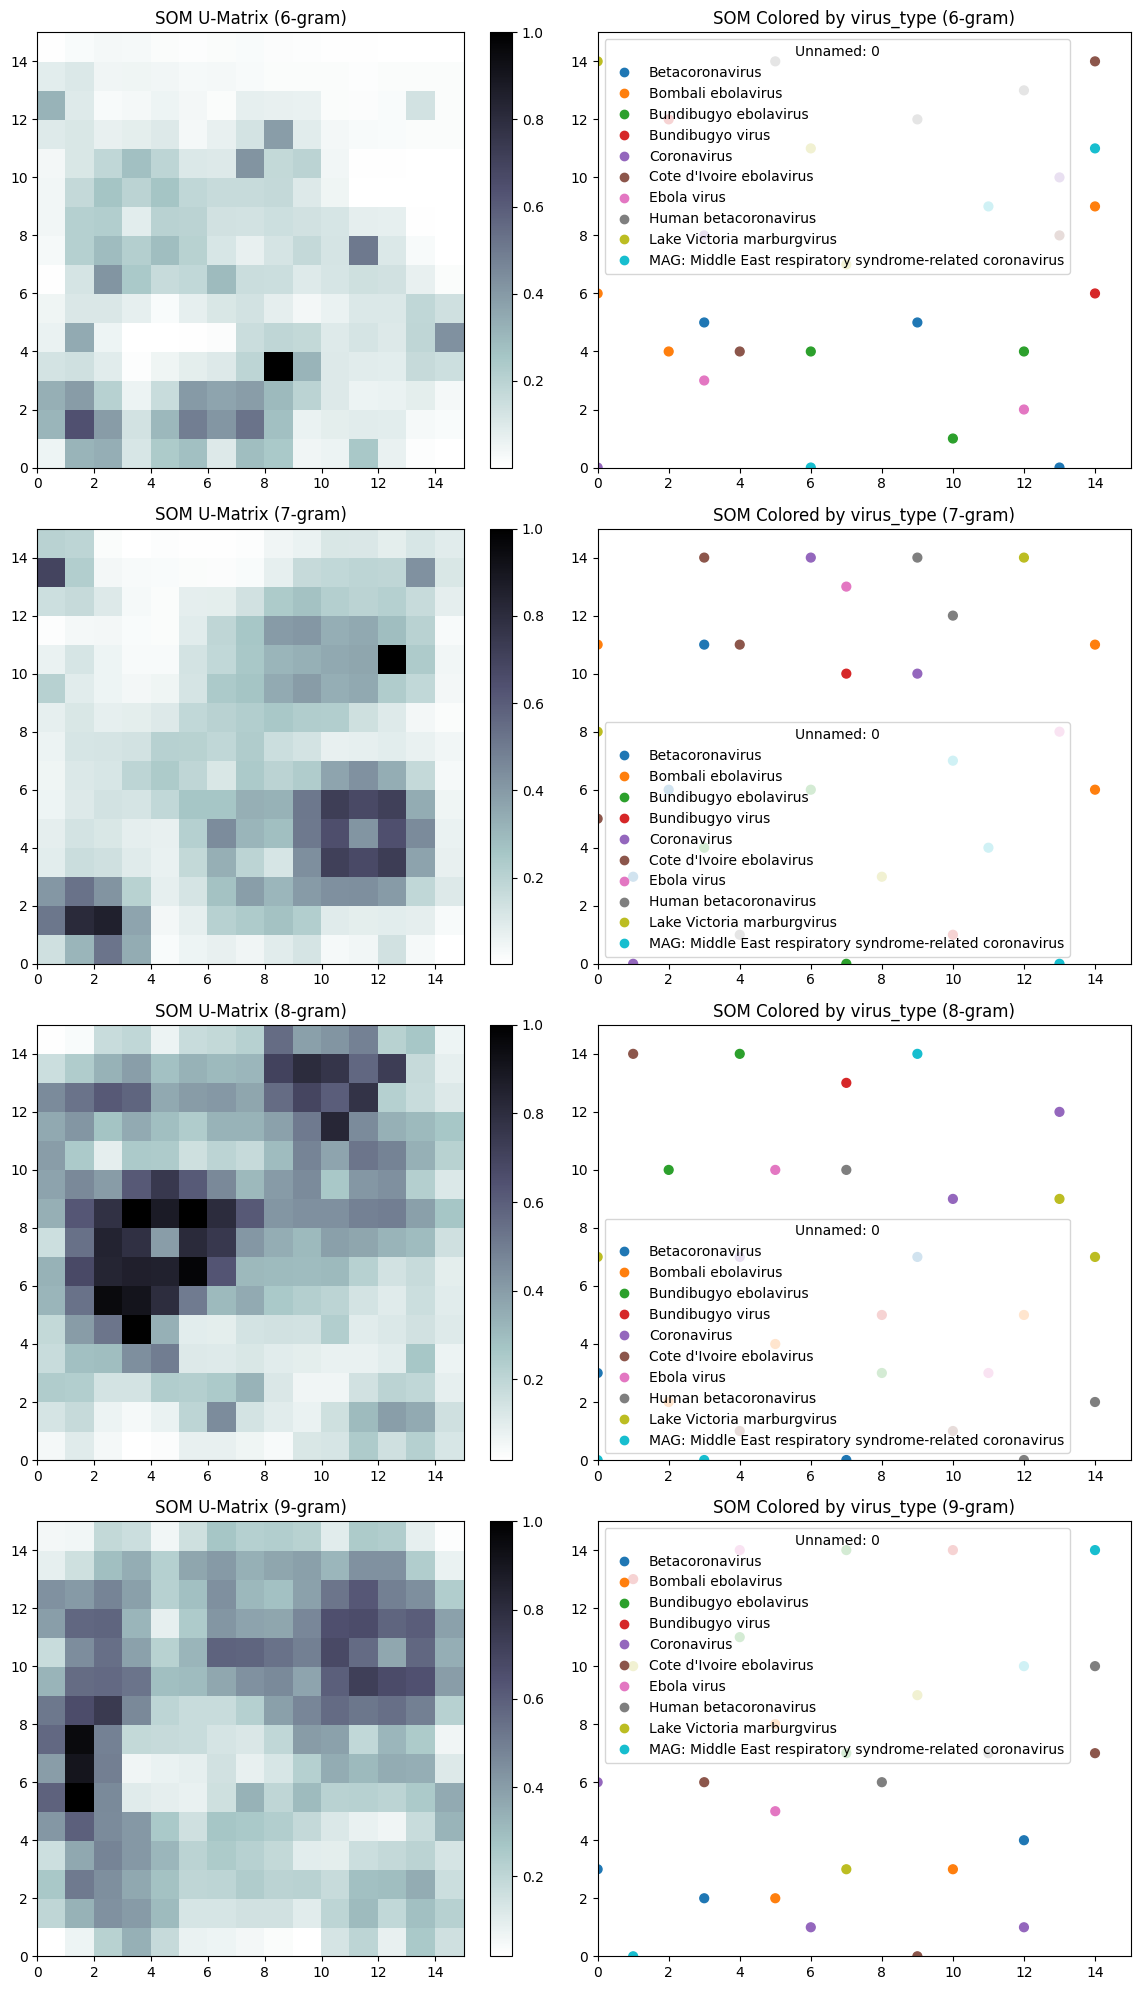
\includegraphics[width=0.5\textwidth]{images/nucleotide-virus.png}
    \caption{Vizualizacija za grupisanje prema tipu virusa}
    \label{fig:som-struktura1}
\end{figure}

\textbf{Slika 3:} Primer rezultata za nukleotidne sekvence – SOM projekcija na osnovu 6-mer frekvencijskih profila
kompletnog genoma. Svaka tačka predstavlja jedan virusni genom, obojen prema tipu virusa (legenda
desno: različite boje za SARS-CoV-2, MERS, različite vrste ebolavirusa i marburgvirusa). Uočljivo je grupisanje
genoma iste virusne vrste u kompaktnije klastere. Na primer, genomi ebolavirusa (različitih sojeva/species)
mapirani su blizu jedni drugih (zelene nijanse), dok su koronavirusi (plave nijanse) razdvojeni u drugi deo
mape. Ovakvi rezultati potvrđuju da matrice n-gram frekvencija, konstruisane opisanim postupkom
parsiranja i obrade podataka, predstavljaju dobru osnovu za primenu SOM algoritma i efikasno
klasterovanje viralnih sekvenci. Kao i za 6-grame, i kod 7-grama, 8-grama i 9-grama uočavaju se izraženija razdvajanja i jasnije formirani klasteri, ali se sa porastom broja n ujedno šire i prazni delovi mape, što ukazuje na sve ređu pokrivenost prostora sekvencama.

\vspace{200pt}
\textbf{Zaključak:}

\vspace{10pt}
\textbf{SOM algoritam} se pokazao kao efikasan i interpretabilan metod za nadozorovano klasterovanje kako proteinskih, tako i genetskih sekvenci. Njegova sposobnost da projektuje podatke u 2D prostor i da očuva topološku strukturu omogućila nam je da:

\begin{itemize}
    \item Identifikujemo grupe sličnih sekvenci prema tipu virusa i tipu proteina.
    \item Uočimo evolutivno povezane sekvence, čak i između različitih virusa.
    \item Potvrdimo da n-gramski profil predstavlja pouzdanu reprezentaciju za bioinformatičko klasterovanje.
\end{itemize}

\newpage
\subsection{Hijerarhijsko klasterovanje}

Hijerarhijsko klasterovanje: Nakon HDBSCAN analize, primenile smo aglomerativno hijerarhijsko
klasterovanje (metod najbližeg suseda / Wardove metode) na iste skupove podataka (6-gram do 9-gram).
Cilj je bio da potvrdimo nalaze i odredimo optimalan broj klastera pomoću metrika validacije. Izračunate su
tri metrike za svaki mogući broj klastera k od 2 do 10: silueta, Calinski-Harabasz indeks i Davies-
Bouldin indeks. Silueta ocenjuje homogenost klastera i njihovu separaciju (viša vrednost je bolja) ; Calinski-Harabasz (CH) indeks računa odnos između-varijacije i unutar-varijacije (takođe veći je bolji za jasno
razdvojene klastere) ; Davies-Bouldin (DB) indeks meri prosečnu „sličnost” svakog klastera sa njemu
najsličnijim susednim klasterom (niža vrednost znači bolju separaciju) . Grafikoni ovih metrika u funkciji
broja klastera $k$ prikazani su za svaki n-gram profil (4 grafa po metriku, za 6,7,8,9-gram). Posmatrajući
grafikone, uočile smo da je za 6-gram podatke metrika siluete bila najveća za otprilike 5 klastera, što se
poklapa sa HDBSCAN rezultatom od 5 klastera. Istovremeno, Calinski-Harabasz indeks je pokazivao lokalni
maksimum u tom području, a Davies-Bouldin minimum, potvrđujući da je podela na 5 grupa najrazumnija
za 6-mer profile. Nasuprot tome, za 7-gram, 8-gram i 9-gram grafici su sugerisali manje brojeve klastera, 
tipično silueta je bila najveća za 2 ili 3 klastera, dok bi CH indeks takođe tu negde imao prelom (elbow). Ove
metrike dakle podržavaju zaključak da sa dužim n-gramima podaci efekivno formiraju dve glavne grupe
(plus eventualno treću manju). Mi smo se odlučile da kao optimalan broj klastera uzmemo k=3 za dalje
analize, kao kompromis koji obuhvata glavnu podelu (filovirusi vs. koronavirusi) ali i dozvoljava mogućnost
odvajanja treće grupe (npr. Marburg ili određeni outlier).

\subsubsection{Nad amino-kiselinskim sekvencama}

\noindent
\begin{minipage}{\textwidth}
Hijerarhijsko klasterovanje za 3-gram, 4-gram i 5-gram profile prikazano je pomoću tri evaluacione metrike 
(silhouette, Calinski–Harabasz i Davies–Bouldin indeksi) u funkciji broja klastera $k$ od 2 do 10. Kod svih profila 
silueta dostiže maksimum pri manjem broju klastera (2–3), a zatim postepeno opada, što ukazuje na to da je struktura 
podataka relativno kompaktna i da manji broj grupa obezbeđuje jasnije granice. Calinski–Harabasz indeks takođe naglo 
opada nakon $k=2$, sugerišući da dodatno povećanje broja klastera ne poboljšava razdvajanje među njima. Davies–Bouldin 
indeks je najniži pri $k=2$ ili $k=3$, potvrđujući da je tu separacija među grupama najveća. Ovi rezultati konzistentno 
sugerišu da za sve tri dužine n-grama optimalan broj klastera leži u rasponu od 2 do 3, što se uklapa u očekivanje da kraći 
n-grami još uvek grupišu podatke u relativno grube, ali stabilne kategorije.
\end{minipage}

\begin{figure}[h!]
    \centering
    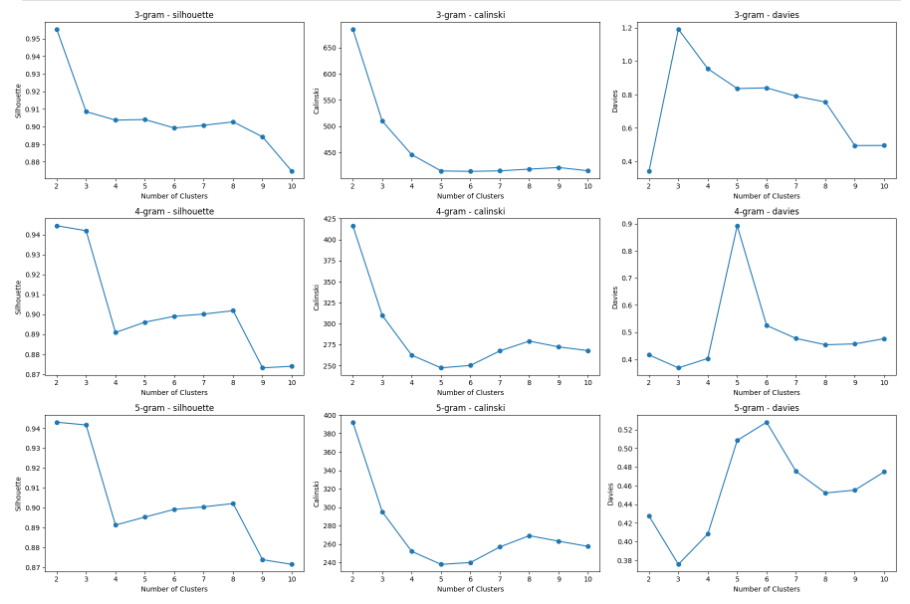
\includegraphics[width=1\textwidth]{images/hcamino.png}
    \caption{Odnos mtrika i broja klastera za sve n-grame}
    \label{fig:hc_aa_metricks}
\end{figure}

\noindent
\begin{minipage}{\textwidth}
Na slici 5 prikazana je PCA projekcija n-gram karakteristika ($3-$, $4-$ i $5-$gram), gde su tačke obojene prema virusnim etiketama (virus\_type), uz obeležene klastere dobijene hijerarhijskim klasterovanjem za $k=3$. Kod 3-gram profila klasteri su manje kompaktni, sa delimičnim preklapanjem između porodica, mada se već naziru dve glavne grupacije – filovirusi (nijanse narandžaste, crvene i zelene) i koronavirusi (nijanse plave i ljubičaste). Kod $4-$grama grupisanje postaje jasnije: jedan klaster obuhvata isključivo filoviruse, drugi koronaviruse, dok je treći manji i okuplja nekoliko izdvojenih sekvenci. Kod $5-$grama klasteri su vrlo zbijeni, sa gotovo potpunim razdvajanjem između glavnih porodica, ali uz tendenciju da se razlike između blisko srodnih virusa unutar iste porodice smanje. Generalno, klasterovanje n-gram profila po virusnom tipu pokazuje da su genomske sekvence srodnih virusa grupisane zajedno, što odražava njihove zajedničke evolucione i statističke obrasce u raspodeli nukleotida.
\end{minipage}

\begin{figure}[h!]
    \centering
    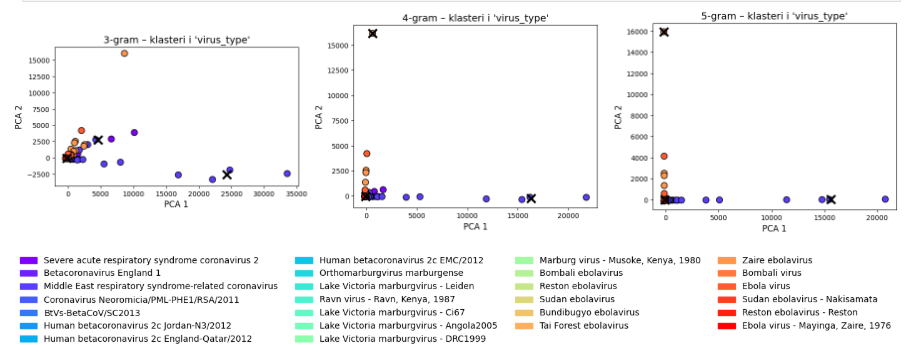
\includegraphics[width=1.2\textwidth]{images/hcvirusaa.png}
    \caption{Odnos mtrika i broja klastera za sve n-grame}
    \label{fig:hc_virus}
\end{figure}

\noindent
\begin{minipage}{\textwidth}
Na drugom setu grafika (slika 6) prikazana je PCA projekcija n-gram karakteristika (3-, 4- i 5-gram) obojenih prema proteinskim etiketama (protein\_type), uz iste parametre klasterovanja ($k=3$). Za razliku od razdvajanja po virusima, ovde je preklapanje znatno veće, jer proteini istog tipa mogu postojati kod filovirusa i koronavirusa, pa genomski profil proteina ne mora biti jedinstven za jednu virusnu porodicu. Kod 3-grama tačke su znatno raspršenije i klasteri manje jasni. Kod 4-grama uočava se bolja kompaktnost i delimično razdvajanje proteinskih grupa, dok 5-gram dovodi do najzbijenijih klastera, ali uz smanjenu vidljivost razlika između srodnih proteina. Ovakav obrazac ukazuje da je n-gram pristup efikasniji za razdvajanje sekvenci po virusnom tipu nego po tipu proteina, jer su proteini često konzervisani između različitih virusa i dele slične n-gram frekvencijske obrasce.
\end{minipage}

\begin{figure}[h!]
    \centering
    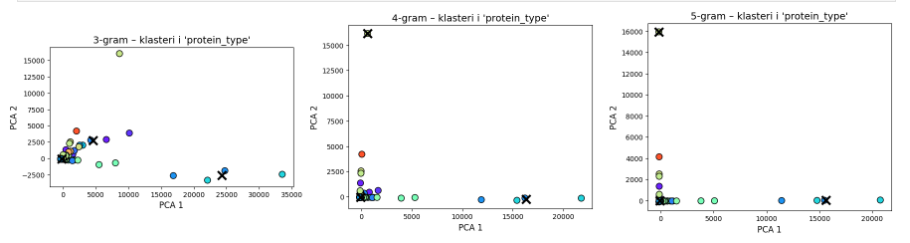
\includegraphics[width=1.2\textwidth]{images/hcproteinaa.png}
    \caption{Vizualizacija}
    \label{fig:hc_protein}
\end{figure}

\noindent
\begin{minipage}{\textwidth}
Dendogram (slika 7): Na ranim nivoima spajaju se sekvence istog virusa.
Srednji nivoi konsoliduju unutar-virusne grupe u veće grane po virusnoj porodici.
Kasni nivoi spajaju velike grane (filovirusi - koronavirusi).
Povećanje n-grama produžava razdaljine između glavnih grana i pojačava separaciju.
\end{minipage}

\begin{figure}[h!]
    \centering
    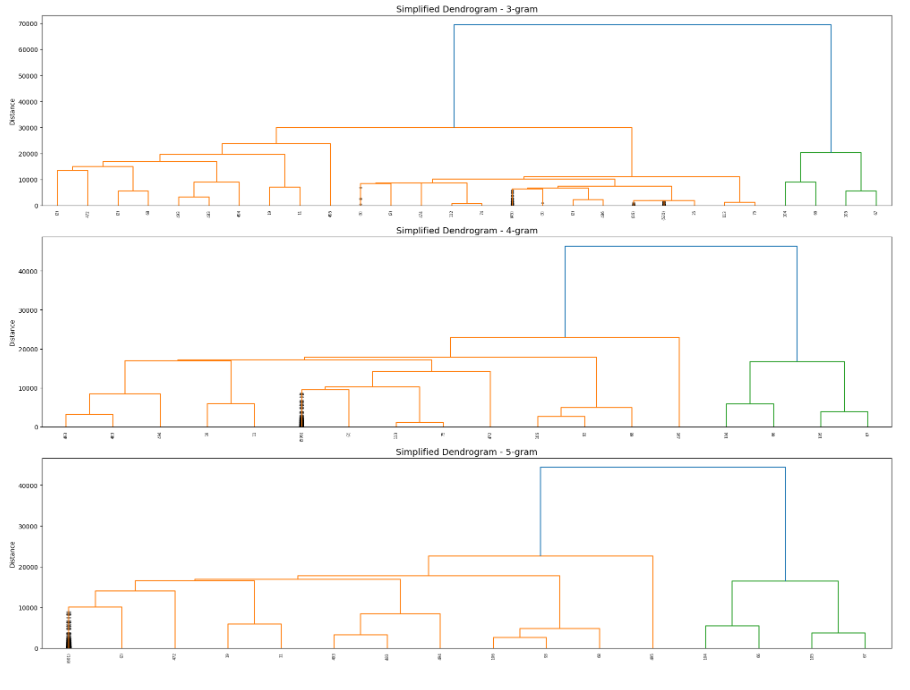
\includegraphics[width=1\textwidth]{images/hcdenaa.png}
    \caption{Dendogram}
    \label{fig:hc_dend}
\end{figure}

\newpage
\subsubsection{Nad nukleotidnim sekvencama}


Primenile smo aglomerativno hijerarhijsko
klasterovanje (metod najbližeg suseda / Wardove metode) na iste skupove podataka (6-gram do 9-gram).
Cilj je bio da potvrdimo nalaze i odredimo optimalan broj klastera pomoću metrika validacije. Izračunate su
tri metrike za svaki mogući broj klastera $k$ od 2 do 10: silueta, Calinski-Harabasz indeks i Davies-
Bouldin indeks. Silueta ocenjuje homogenost klastera i njihovu separaciju (viša vrednost je bolja) ; Calinski-Harabasz (CH) indeks računa odnos između-varijacije i unutar-varijacije (takođe veći je bolji za jasno
razdvojene klastere) ; Davies-Bouldin (DB) indeks meri prosečnu „sličnost” svakog klastera sa njemu
najsličnijim susednim klasterom (niža vrednost znači bolju separaciju) . Grafikoni ovih metrika u funkciji
broja klastera $k$ prikazani su za svaki n-gram profil (4 grafa po metriku, za 6,7,8,9-gram). Posmatrajući
grafikone, uočile smo da je za 6-gram podatke metrika siluete bila najveća za otprilike 5 klastera, što se
poklapa sa HDBSCAN rezultatom od 5 klastera. Istovremeno, Calinski-Harabasz indeks je pokazivao lokalni
maksimum u tom području, a Davies-Bouldin minimum, potvrđujući da je podela na 5 grupa najrazumnija
za 6-mer profile. Nasuprot tome, za 7-gram, 8-gram i 9-gram grafici su sugerisali manje brojeve klastera –
tipično silueta je bila najveća za 2 ili 3 klastera, dok bi CH indeks takođe tu negde imao prelom (elbow). Ove
metrike dakle podržavaju zaključak da sa dužim n-gramima podaci efekivno formiraju dve glavne grupe
(plus eventualno treću manju). Mi smo se odlučile da kao optimalan broj klastera uzmemo $k=3$ za dalje
analize, kao kompromis koji obuhvata glavnu podelu (filovirusi vs. koronavirusi) ali i dozvoljava mogućnost
odvajanja treće grupe (npr. Marburg ili određeni outlier).

\begin{figure}[h!]
    \centering
    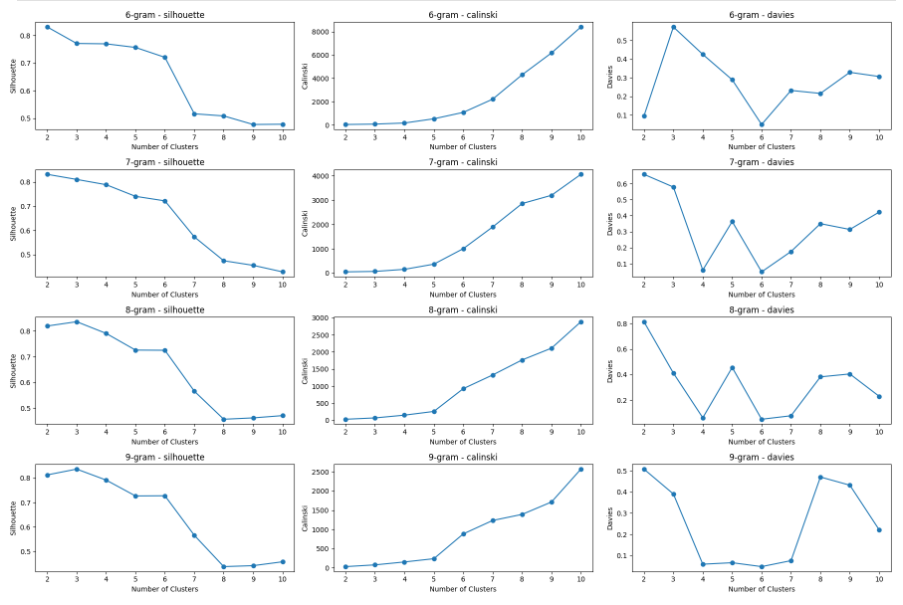
\includegraphics[width=1.2\textwidth]{images/hc_metrika_nuk.png}
    \caption{Odnos mtrika i broja klastera za sve n-grame}
    \label{fig:hc_met_nuk}
\end{figure}

Na slici ispod (slika 9) prikazana je PCA projekcija 6-gram karakteristika, gde su tačke obojene prema virusnim
etiketama (tipovima virusa), uz obeležene klastere dobijene hijerarhijskim klasterovanjem za $k=3$. Jasno se
vidi da postoji jedna grupacija (klaster) koja sadrži isključivo tačke označene bojama koje predstavljaju
filoviruse (nijanse iste palete za različite Ebola vrste, plus jedna za Marburg), dok je druga grupacija tačaka
(drugi klaster) u potpunosti druge boje – to su koronavirusi. Treći klaster je bio vrlo mali i u ovom primeru je
obuhvatio samo jednu ili dve tačke (zavisno od $k$ preseka), što bi odgovaralo nekoj izdvojenoj sekvenci ili
noise grupi. Generalno, klasterovanje nukleotidnih n-gram profila virusa grupisalo je genomske
sekvence prema porodici i rodu virusa, što znači da su virusi srodnih tipova imali slične obrasce n-gram
frekvencija. Ovakav rezultat je u skladu sa očekivanjem da evolucioni srodni virusi dele određene statističke
osobine genoma (npr. sličan sadržaj baza i dinukleotidne preferencije), čime se razlikuju od udaljenijih
grupa.

\begin{figure}[h!]
    \centering
    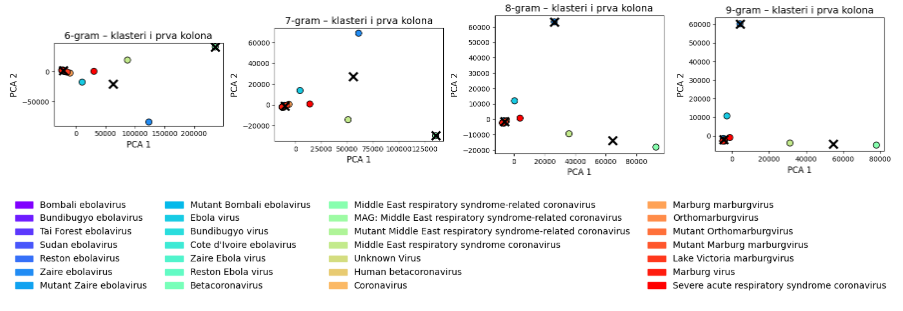
\includegraphics[width=1.2\textwidth]{images/hc_nuk.png}
    \caption{Vizualizacija}
    \label{fig:hc_nuk}
\end{figure}

Izvršile smo vizuelizaciju hijerarhijskog klasterovanja tako što smo nacrtale simplifikovane dendograme i projekcije podataka sa označenim klasterima. Dendrogrami (trunkovani na nivou 6 radi preglednosti) su jasno pokazali odvajanje dve velike grane – jedna koja je sadržala sve filoviruse (Ebola i Marburg pod-grane), i druga sa koronavirusima – potvrđujući da je ta podela najdominantnija u podacima. Na nižim nivoima dendrograma
videlo se dalje grananje filovirusa na pojedinačne vrste Ebola virusa, što odgovara očekivanom filogenetskom razdvajanju. Dakle, hijerarhijsko klasterovanje nije samo potvrdilo nalaze HDBSCAN-a, već je i pružilo hijerarhijski kontekst – npr. pokazalo je da su svi ebolavirusi prvo grupisani zajedno pre nego što se priključe marburgvirusima na višem nivou (Filoviridae), što se zatim tek na najvišem nivou spaja sa klasterom koronavirusa (što odgovara razlici između Filoviridae i Coronaviridae).

\begin{figure}[h!]
    \centering
    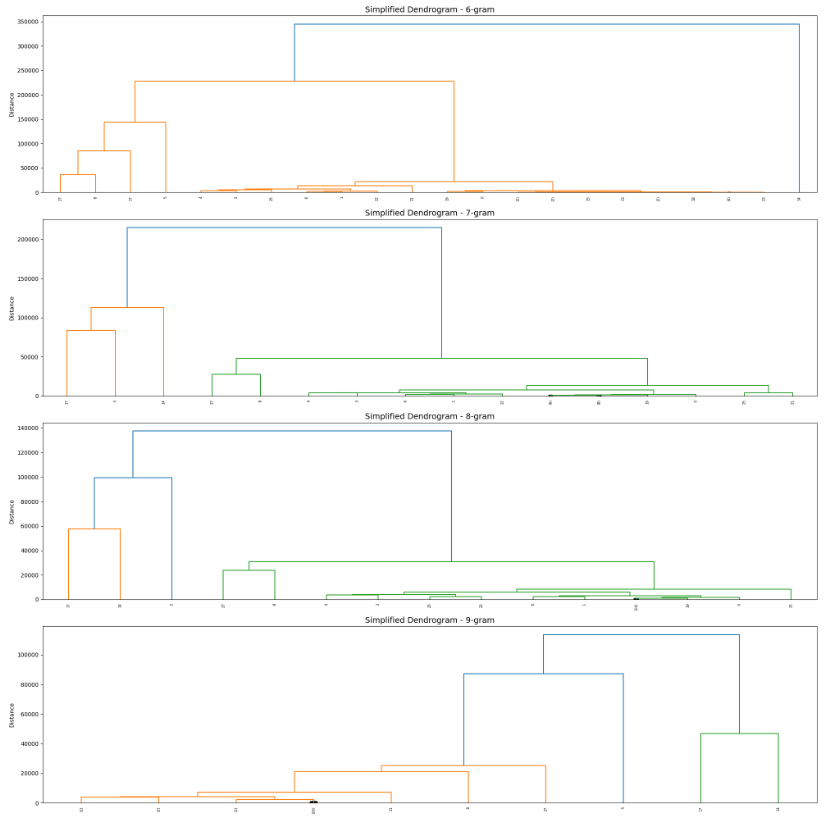
\includegraphics[width=1.2\textwidth]{images/hc_den_nuk.png}
    \caption{Dendogram}
    \label{fig:hc_ded}
\end{figure}

\newpage
\subsection{K-Means}
K-Means klasterovanje je korišćeno za skup amino-kiselinskih sekvenci. Iako zahteva da se unapred zada broj klastera k, K-Means je jednostavan i veoma brz algoritam koji efikasno skalira na veće skupove podataka . U našem slučaju, dimenzionalnost vektora amino-kiselinskih n-grama (3-grama, 4-grama, 5-grama) je relativno velika, ali K-Means uspešno može da grupiše podatke tako da minimizira varijansu unutar klastera. Poznato je da K-Means daje najbolje rezultate kada su klasteri globularni (sferni) i relativno uravnoteženi po veličini, što smo pretpostavili kao razumno približenje za amino-kiselinske profile virusa. Dodatno, K-Means ima prednost brzog računanja i lakog ponavljanja za različite k, što nam omogućava da primenimo metode za određivanje optimalnog broja klastera (npr. metod „lakta“ i koeficijent siluete). K-Means je generalno popularan u bioinformatici za osnovno grupisanje sekvenci ili osobina jer je jednostavan za primenu i brzo konvergira.

\subsubsection{Nad amino-kiselinskim sekvencama}
\noindent
\begin{minipage}{\textwidth}
Kao što je pomenuto, K-Means zahteva unapred definisan broj klastera k, pa smo prvo primenile metod silueta i srodne metrike da bismo odabrale k. Isprobale smo vrednosti $k=2$ do 10 za svaki skup (3-gram, 4-gram, 5-gram) i izračunale prosečnu siluetu, Calinski-Harabasz i Davies-Bouldin indekse. Sve tri metrike su uglavnom sugerisale da je k=3 optimalan ili blizu optimalnog za sve tri veličine n-grama (kod 3-grama se takođe k=4 javljao kao moguće rešenje prema CH kriterijumu, ali silueta je opadala za k>3). Odlučile smo se za tri klastera kao zajednički broj koji dobro opisuje strukturu podataka u sva tri skupa n-grama, radi konzistentnosti interpretacije. Vredi napomenuti da je u ovoj analizi broj klastera relativno mali, što odgovara našem očekivanju da se proteini možda grupišu u nekoliko glavnih kategorija.
\end{minipage}

\begin{figure}[H]
    \centering
    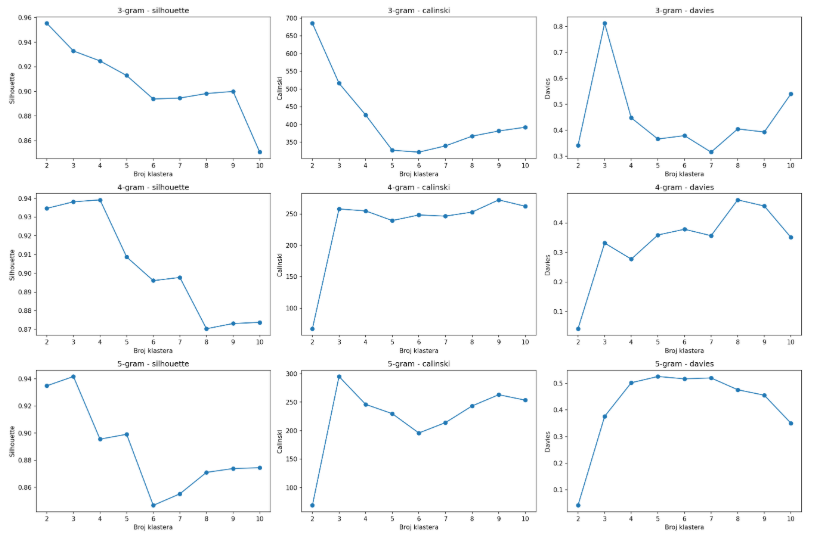
\includegraphics[width=1.2\textwidth]{images/km_met.png}
    \caption{Odnos mtrika i broja klastera za sve n-grame}
    \label{fig:km_met}
\end{figure}

\noindent
\begin{minipage}{\textwidth}
Nakon određivanja broja klastera, K-Means algoritam je pokrenut (sa k=3 i inicijalizacijom ponovljenom više puta radi stabilnosti). Rezultujući klasteri su analizirani na dva načina: (1) posmatrali smo klastere s obzirom na tip virusa odakle potiče protein, i (2) s obzirom na vrstu proteina (funkciju proteina). Ideja je bila da odgovorimo na pitanje: Da li se proteinske sekvence grupišu prvenstveno prema tome kom virusu pripadaju ili prema tome koju ulogu/protein predstavljaju?
\end{minipage}

\vspace{1cm}

\noindent
\begin{minipage}{\textwidth}
Dobijeni klasteri u prostoru glavnih komponenti prikazani su na slikama ispod. Prva slika prikazuje projicirane proteine obojene prema virusnom tipu (npr. svi proteini iz koronavirusa jedne boje, iz ebolavirusa druge, itd.), dok druga slika prikazuje iste klastere ali sa bojama prema vrsti proteina (npr.glikoproteini jedne boje, polimeraze druge, nukleoproteini treće itd.). Crnim znakom "X" označeni su centri klastera koje je odredio K-Means algoritam u prostoru prve dve komponente PCA.
\end{minipage}

\begin{figure}[H]
    \centering
    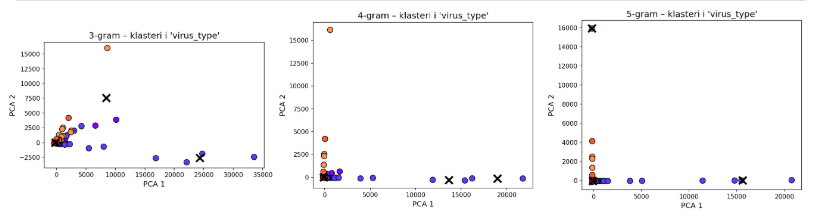
\includegraphics[width=1.2\textwidth]{images/km_virus.png}
    \caption{Odnos mtrika i broja klastera za sve n-grame}
    \label{fig:km_vir}
\end{figure}

Slika 12: Klasterovanje proteina virusa prema amino-kiselinskim n-gram profilima (3-gram, 4-gram, 5-gram). Prikazan je PCA grafikon za svaku dimenziju n-grama (kolone grafikona), gde su tačke obojene prema tipu virusa odakle potiče dati protein. Crni znaci "X" označavaju centri klastera dobijenih K-Means algoritmom za k=3. Uočava se da su proteini grupisani tako da većina proteina iz iste virusne porodice (isti koloritet) leži u istom klasteru. (Primjer: narandžaste i ljubičaste tačke – koje predstavljaju različite vrste Ebola virusa – čine jedan klaster levo, zelene i plave tačke – koje predstavljaju koronaviruse – čine drugi klaster desno.)

\begin{figure}[H]
    \centering
    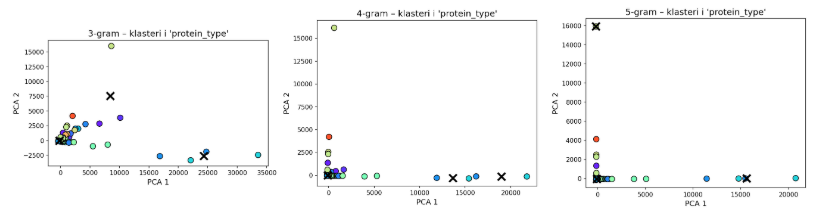
\includegraphics[width=1.2\textwidth]{images/km_protein.png}
    \caption{Odnos mtrika i broja klastera za sve n-grame}
    \label{fig:km_prot}
\end{figure}


\noindent
\begin{minipage}{\textwidth}
Slika 13: Isti klasteri kao na Sl. 12, ali su tačke obojene prema tipu proteina (funkcionalnoj klasifikaciji proteina). Oznake boja: npr. zelena boja = glikoproteini (GP) različitih virusa, plava = polimerazni lanci (npr. L protein Ebola virusa, ili polimeraza koronavirusa), crvena = nukleokapsidni proteini itd. Vidljivo je da unutar istog klastera postoje raznobojne tačke, što znači da klasteri sadrže više različitih vrsta proteina – nisu se grupisali proteini istog tipa, već pretežno proteini istog virusa.
\end{minipage}

\vspace{1cm} 

Konkretno, u rezultatima vidimo da je jedan klaster obuhvatio sve proteine filovirusa (različite boje u tom klasteru na Sl. 2 predstavljaju GP, NP, VP35 itd. iz Ebola/Marburg virusa), dok je drugi klaster obuhvatio sve proteine koronavirusa (opet različite funkcije, ali svi potiču od korona virusa). Treći klaster je bio malobrojan i uključivao je eventualno proteine iz neke treće grupe virusa ako je bila zastupljena (u našem skupu moguće ako smo imali predstavnika druge porodice, ili je pak treći klaster činio outlier). Ovakav ishod je očekivan, jer su sekvence proteina unutar istog virusa relativno konzervativne u pogledu kompozicije, dele specifičan obrazac aminokiselinske zastupljenosti (uslovljen genomom i stilom kodiranja tog virusa), dok isti tipovi proteina između filogenetski udaljenih virusa (npr. površinski glikoproteini Ebola vs. korona) nemaju sličnost u primarnoj strukturi koja bi ih grupisala. Zapravo, rezultati impliciraju da je signal virusne pripadnosti jači od signala proteinske funkcije u prostoru n-gram frekvencija.

\vspace{1cm}

\noindent
\begin{minipage}{\textwidth}
Ovo zapažanje možemo povezati sa biološkim činjenicama: proteini jednog virusa evoluiraju zajedno i svi su pod uticajem globalnih svojstava tog virusa (npr. nukleotidnog sastava genoma, stope mutacija, pritiska imunog sistema domaćina, mehanizama replikacije itd.), što može dovesti do toga da i različiti proteini tog virusa imaju slične statističke osobine (aminokiselinski sastav, preferencije dipeptida, itd.). Nasuprot tome, isti tip proteina kod različitih virusa (recimo, RNA polimeraza kod RNK virusa) može deliti određene katalitičke motive na sekvenci, ali će veliki deo sekvence biti različit zbog dugog nezavisnog evoluiranja – stoga njihov n-gram profil neće biti dovoljno sličan da bi ih K-Means spojio u isti klaste
\end{minipage}

\begin{figure}[H]
    \centering
    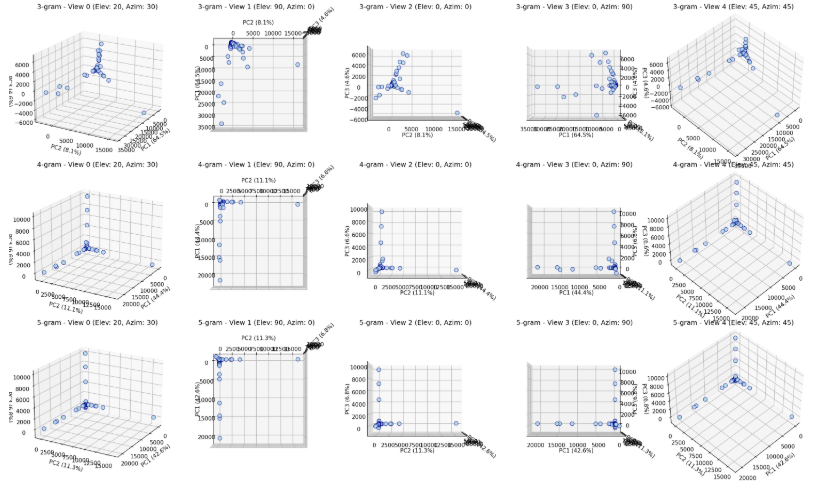
\includegraphics[width=1.2\textwidth]{images/3d.png}
    \caption{Odnos mtrika i broja klastera za sve n-grame}
    \label{fig:3d}
\end{figure}

Slika 14 prikazuje 3D projekciju podataka nakon PCA analize. Svaka tačka predstavlja jedan uzorak, a njena pozicija određena je vrednostima u tri glavne komponente (PC1, PC2, PC3), koje zadržavaju najveći deo varijanse podataka. Prikaz iz više uglova omogućava uočavanje prirodnih grupa i raspodele uzoraka, iako eksplicitno klasterovanje nije izvršeno.

\subsection{HDBSCAN}

HDBSCAN je metoda zasnovana na gustini koja automatski određuje broj klastera na osnovu strukture
podataka, bez potrebe da se unapred zada k. To ga čini pogodnim za kompleksne skupove podataka
sa nepoznatim brojem grupa i neravnomernom gustinom tačaka. Takođe, HDBSCAN može da otkrije
klastere nepravilnih oblika i da izdvoji šum (outlier podatke) kao posebnu kategoriju , što je korisno kod
bioloških podataka gde neki virusi mogu biti jedinstveni i ne pripadaju nijednoj grupi. U našem slučaju,
vektori karakteristika (n-gram frekvencije) mogu imati kompleksnu strukturu, pa je prednost HDBSCAN-a
što identifikuje stabilne klastere različitih oblika i veličina bez stroge pretpostavke o raspodeli podataka.
Pored toga, HDBSCAN internim postupkom gradi hijerarhiju klastera (dendrogram zasnovan na
minimalnom raspinjućem drvetu), što omogućava uvid u strukturu grupisanja na više nivoa granularnosti.
Ovakav pristup je u skladu sa savremenim metodama za grupisanje genetičkih sekvenci – na primer,
alat ViralClust koristi k-mer reprezentaciju genoma i HDBSCAN (u kombinaciji sa UMAP projekcijom) za
grupisanje virusa po sličnosti genoma.

\subsubsection{Nad nukleotidnih sekvencama}

Algoritam je pronašao jasne klastere među virusnim genomima. Konkretno, za 6-gram
profile identifikovano je 5 klastera (plus određeni broj šumskih tačaka koje nisu pripale nijednom klasteru),
dok je za više vrednosti $n$ (7-gram, 8-gram, 9-gram) uglavnom detektovao 2 klastera uz veći udeo šuma.
Ovaj trend sugeriše da kraći n-grami (6-meri) nose dovoljno informacija da razlikuju više finih grupa virusa,
dok duži n-grami (poput 9-mera) daju vrlo specifične profile zbog kojih se virusi grupišu samo u grublje
kategorije, a mnogi specifični virusi ostaju izdvojeni kao šum. Kvalitet klasterovanja meren je koeficijentom
silhouette – za 6-grame dobijena je prilično visoka prosečna silueta (~0.43), što ukazuje na dobro odvojene
klastere. Za 7-grame i duže, silueta je bila niža (~0.20–0.23), u skladu sa činjenicom da je algoritam tu
uglavnom pronašao samo dva klastera i veliki broj izdvojenih tačaka (što smanjuje prosečnu siluetu). Ovo
može značiti da se sa porastom dužine n-grama viralni genom postaje toliko jedinstven da HDBSCAN
prepoznaje samo dve velike grupe (moguće podela na dve velike familije virusa) i tretira ostale kao dovoljno
različite (noise) ili ih uključuje u te grupe sa manjom pouzdanošću.

%SLIKA ZA HDBSCAN SA NOVIM PARAMETRIMA I SLIKA TABELE GDE PISE SILUETA

\noindent
\begin{minipage}{\textwidth}
\textbf{Diskusija}: Važno je napomenuti da HDBSCAN ne zahteva odabir parametra $k$, već parametre minimalne veličine klastera i slično. Mi smo koristile relativno konzervativne vrednosti (min\_cluster\_$size = 2$, min\_samples$ = 1$)
kako bismo omogućile detekciju i manjih grupa. Detektovani klasteri pokazali su jaku korelaciju sa
taksonomijom virusa. Analizom oznaka sekvenci (prva kolona dataseta predstavljala je tip ili naziv virusa)
utvrdile smo da su, na primer, genomi različitih ebolavirusa grupisani zajedno, odvojeno od genoma
koronavirusa. HDBSCAN je, dakle, uspeo da automatski izdvoji familije virusa na osnovu n-gram sastava
njihovih genoma. Za 6-grame, pet identifikovanih klastera približno su odgovarali: (1) grupa ebolavirusa
(različite vrste Ebola virusa poput Zair, Sudan, Bundibugyo i sl. zajedno), (2) Marburg virus (blizak Ebola
virusima ali dovoljno različit da čini poseban klaster), (3) grupu koronavirusa (različiti beta-koronavirusi,
uključujući MERS, SARS i sl.), i preostale manje grupe povezane sa drugim rodovima. Ovakva podela
reflektuje biološku stvarnost – filovirusi (Ebola i Marburg) čine jednu nad-grupu, dok koronavirusi čine
drugu, s tim da unutar filovirusa postoje podgrupe među vrstama ebolavirusa. Za veće $n$ (7–9), HDBSCAN
je nalazio samo po 2 klastera – u suštini je grupisao sve filoviruse u jedan klaster, a sve koronaviruse u drugi,
dok su neki pojedinačni virusi ostajali označeni kao šum. To indicira da su 7–9-mer frekvencije toliko
specifične da ističu samo grubu podelu (verovatno prema familijama virusa), dok fine razlike među srodnim
virusima (npr. različite vrste ebolavirusa) više ne formiraju stabilne klastere za datu konfiguraciju
parametara.
\end{minipage}
\vspace{1cm}

Uz vizuelizaciju pomoću PCA, mogle smo da prikažemo tačke (genome) u 2D prostoru bojene prema pravim etiketama (tipovima virusa) i da označimo klastere dobijene HDBSCAN-om. Ti scatter grafici su potvrdili da
su tačke istih virusnih grupacija završile blizu jedna druge i u istom klasteru. Klasteri su imali biološku
interpretaciju: npr. svi ebolavirusi bili su blizu i dodeljeni jednom klasteru, odvojeni od klastera koji je obuhvatao koronaviruse. Marburg virus se u nekim analizama izdvajao kao poseban mali klaster ili kao noise, zavisno
od parametara, što opet ima smisla jer je filovirus ali dosta divergentan od ebolavirusa. Ovi nalazi
demonstriraju da n-gram profil genoma nosi signal koji odgovara virusnoj klasifikaciji, što je u skladu s
drugim studijama gde su k-mer pristupi korišćeni za taksonomsko grupisanje genoma.
\vspace{1cm}

\noindent
\begin{minipage}{\textwidth}
\textbf{Zakljucak:} Primena HDBSCAN algoritma na n-gram profile virusnih genoma pokazala je da kraći n-grami (6-meri) omogućavaju detekciju više finih klastera, dok duži n-grami (7–9-meri) ističu samo grubu podelu na velike familije virusa. Kvalitet klasterovanja, procenjen koeficijentom silhouette, bio je viši za 6-grame, što ukazuje na bolje odvojene grupe. Klasteri su pokazali jaku korelaciju sa taksonomijom virusa: npr. različite vrste ebolavirusa grupisane su zajedno, odvojeno od koronavirusa, dok se Marburg virus ponekad izdvajao kao poseban klaster ili noise. Vizuelizacija PCA potvrđuje da n-gram profil genoma nosi biološki relevantan signal koji omogućava automatsko grupisanje virusnih genoma u skladu sa njihovim familijama i vrstama.
\end{minipage}

\newpage
\begin{thebibliography}{99}

\bibitem{hdbscan_gfg}
Hierarchical Density-Based Spatial Clustering of Applications with Noise (HDBSCAN) - GeeksforGeeks.  
\url{https://www.geeksforgeeks.org/machine-learning/hdbscan/}

\bibitem{viralclust_github}
GitHub - rnajena/viralclust: Small pipeline to cluster viral genomes based on their k-mer content. WiP.  
\url{https://github.com/rnajena/viralclust}

\bibitem{hierarchical_gfg}
Hierarchical Clustering in Machine Learning - GeeksforGeeks.  
\url{https://www.geeksforgeeks.org/machine-learning/hierarchical-clustering/}

\bibitem{kmeans_uc}
K-means Cluster Analysis · UC Business Analytics R Programming Guide.  
\url{https://uc-r.github.io/kmeans_clustering}

\bibitem{kmeans_neptune}
K-Means Clustering Explained - Neptune.ai.  
\url{https://neptune.ai/blog/k-means-clustering}

\bibitem{typing_onehealth}
Typing methods based on whole genome sequencing data | One Health Outlook | Full Text.  
\url{https://onehealthoutlook.biomedcentral.com/articles/10.1186/s42522-020-0010-1}

\bibitem{clustering_metrics_gfg}
Clustering Metrics in Machine Learning - GeeksforGeeks.  
\url{https://www.geeksforgeeks.org/machine-learning/clustering-metrics/}

\end{thebibliography}


\end{document}
